\documentclass[tikz,border=2mm]{standalone}

\usetikzlibrary{arrows,positioning}

\begin{document}

    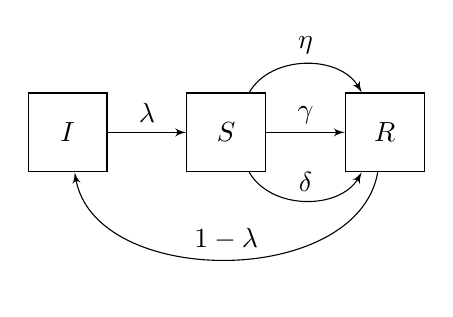
\begin{tikzpicture}[node distance=1cm,auto,>=latex',every node/.append style={align=center},int/.style={draw, minimum size=1cm}]
        \node [int] (I)             {$I$};
        \node [int, right=of I] (S) {$S$};
        \node [int, right=of S] (R) {$R$};
        \path[->, auto=false] (I) edge node {$\lambda$ \\[.2em]} (S) 
        (S) edge node {$\gamma$ \\[.2em]} (R)
        (S) edge  [out=60, in=120] node[above] {$\eta$} (R)
        (S) edge  [out=-60, in=-120] node[above] {$\delta$} (R)
        (R) edge  [out=-100, in=-80] node[above] {$1 - \lambda$} (I);
    \end{tikzpicture}

\end{document}
